\begin{document}

\maketitle

\section{Sissejuhatus}
\begin{frame}[fragile]
  \frametitle{Eelmine kord}
  Peamine fookus IT valitsemisel
	\begin{itemize}
		\item IT valitsemine on naljakas pool-akadeemiline distsipliin. Keeruline kunst.
		\item Äriplaan mõjutab oluliselt arhitektuurseid ja tarkvaratehnilisi otsuseid
		\item Tehniline võlg võib juhtimatuna kergesti tagumikust hammustada
	\end{itemize}
\end{frame}

\begin{frame}[fragile]
  \frametitle{Täna kavas}
		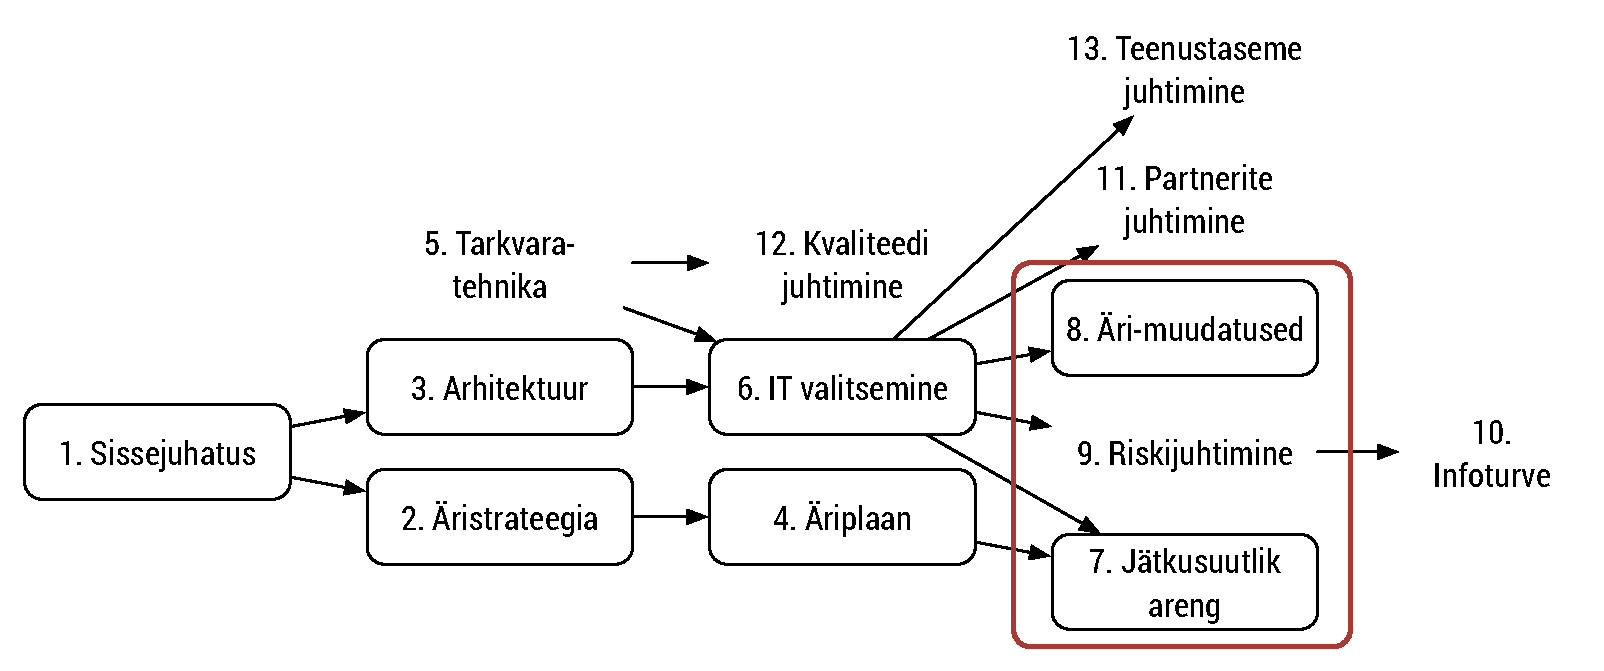
\includegraphics[width=\textwidth]{aine_struktuur_kolmas.pdf}
\end{frame}

\section{Jätkusuutlik areng}
\begin{frame}[fragile]
  \frametitle{Jätkusuutlikkusest}
  	\begin{center}
			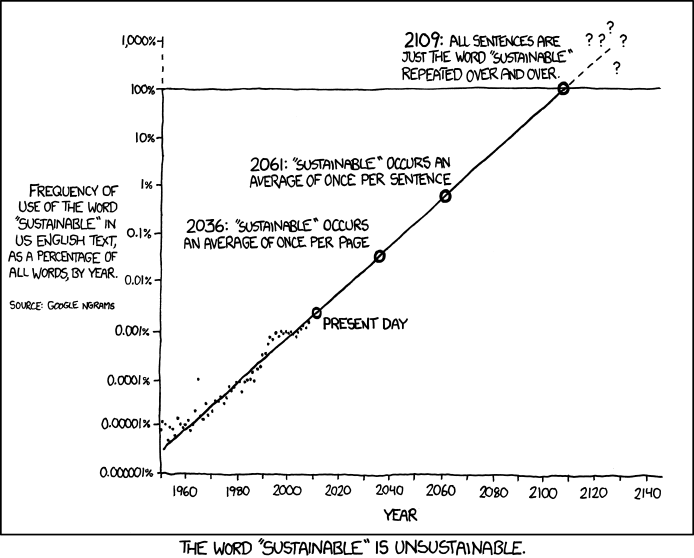
\includegraphics[width=.72\textwidth]{sustainable.png}
	\end{center}
	XKCD 1007
\end{frame}
\note{Jätkusuutlikkuse ümber on väga palju haipi ja vähe fakte. Katsuge näiteks arendada USA ajakirjanduses intelligentset vestlust kliimamuutuse ja selle põhjuste üle: saate sauna mõlemalt poolt. Katsun täna keskenduda jätkusuutlikkuse mõistele ning selle mõjule}

\begin{frame}[fragile]
  \frametitle{Jätkusuutlikkuse definitsioon}
	\begin{itemize}
		\item EKSS: arengu kohta, mis tagab inimeste elukvaliteedi paranemise kooskõlas keskkonna taluvusvõimega
		\item Wikipedia: \emph{sustainability is the endurance of systems and processes}
		\item Kas maasse augu kaevamine on jätkusuutlik tegevus?
		\item Kas 80-tunnine süsadmini töönädal on jätkusuutlik?
	\end{itemize}
\end{frame}

\begin{frame}[fragile]
  \frametitle{Jätkusuutlikkuse definitsioon}
  \begin{center}
  	\begin{quote}
		Jätkusuutlik on tegevus, mida võib mingites ajaraamides sarnaste tulemustega jätkata 
	\end{quote}
  \end{center}

	\begin{itemize}
		\item Laialt levinud definitsioonid on liiga kitsad ning ei ole otse ITle rakendatavad
		\note{Välja arvatud serveriruumide disain}
		\item Mõistes on peidus 
		\begin{itemize}
			\item ajahorisont: ka universum ei ole igavene
			\note{Keskpikas perspektiivis oleme me kõik surnud\par}
			\item ressursi mõiste: tegevuse lõppemise põhjus on ressursi lõppemine
		\end{itemize}
		
		
		\item Meie definitsiooni juured on agiilses tarkvaras \citep{sustainable}
	\end{itemize}
\end{frame}

\begin{frame}[fragile]
  \frametitle{Jätkusuutlikkus kui piirang}
 Vajadust jätkusuutlikkuse järele võib vaadelda kui kõrgemalt strateegia tasemelt seatud piirangut

	\begin{itemize}
		\item Seatakse ka muid piiranguid, neid ei tohi jätkusuutlikkusega segi ajada
		\note{Omanike otsus panna kinni tuumajaamad ja keskenduda hüdroenergiale on samaväärne otsusega mitte maksta altkäemaksu\par}
		\item Piirangud võivad tulla ka mujalt
			\begin{itemize}
				\item Riigilt
				\note{Hollandis peavad suuremahulised maasoojuspumbad näitama viie aasta lõikes null-saldot: maasse pannakse sama palju kui sealt välja võetakse\par}
				\item Kohalikult omavalitsuselt
				\item Maaomanikult
			\end{itemize}
		\item Selles kontekstis on jätkusuutlikkus nagu iga teine organisatsioonile või selle osale seatud piirang
		\note{Kui see on väline, minnakse sellest mööda kui mööda minemise kulu on väiksem, kui reeglite järgimise kulu}
	\end{itemize}
\end{frame}

\begin{frame}[fragile]
  \frametitle{Jätkusuutlikkuse ajahorisont}		
  		Jätkusuutlikkuse põhiline parameeter on ajahorisont, igal organisatsioonil on oma. Startup näeb järgmise raharingini, ülikool sajandite taha.
	  \begin{itemize}
		\item Organisatsiooni ajahorisonti mõjutavad oluliselt
			\begin{itemize}
				\item Kapitali struktuur
				\note{Kui palju on laenu- ja kui palju omanike raha. Kust omanikud raha saavad, kui pikk on laenuraha jne.\par}
				\item Omanike arusaam "väärtusest"
				\note{Iga ettevõtte ülesandeks on maksimeerida omanikele pakutavat väärtust. Börsiettevõtte ajahorisont on praktiliselt üks kvartal.\par}
				\item Keskkond
				\note{Kiiresti muutuvas keskkonnas ei ole võimalik ega mõistlik pikki sihte seada\par}
				\item Organisatsiooni strateegia
				\note{Mõnevõrra juba tulem omanike sisendist, kuid vahel mitte. On raske rääkida rohelisest ITst, kui ettevõtte strateegiaks on leida kõige odavamalt kinni makstavad ametnikud ja nende jurisdiktsioonist kuni vahele jäämiseni väärispuitu välja vedada}
			\end{itemize}		
		\item Iga juhtimistasand seab oma strateegia eelmiselt saadud piirangute alusel lisades omapoolse perspektiivi
		\note{Muude piirangute puudumisel jahutategi te oma serveriruumi hülgepoegadega, kui see juhtub kõige efektiivsem võimalus olema. Samas võib teie ajahorisont piirduda planeeritud tööajaga samas kui organisatsioon vaatab kaugemale\par} 
	\end{itemize}
\end{frame}

%Arutelu koht
\begin{frame}[fragile]
  \frametitle{Arutelu koht}
		\begin{center}
			\textbf{Miks on madal PUE oluline?}
			\note{Power Usage effectivenes}
		\end{center}
\end{frame}

\begin{frame}[fragile]
  \frametitle{Jätkusuutlikkus ja ressursid}
	Mis on see, mis võib otsa saada?

	\begin{itemize}
		\item Materiaalsed ressursid: nafta, gaas, puhas vesi aga ka inimesed
		\item Immateriaalsed ressursid
			\begin{itemize}
				\item Inimesed
				\note{Admini võimekus teha tööd, nende heasoovlikkus\par}
				\item Partnerid
				\note{Parnerite vastutulelikkus, läbirääkimissoov\par}
				\item Regulaatorid
				\note{Politseiniku soov hoiatusega piirduda\par}
				\item Ülemised juhtimistasandid
				\note{Väga oluline! Tippjuhtkond on suuteline oma soovide ignoreerimist taluma vaid piiratud hulga aega!\par}
			\end{itemize}		
		\item Oluline küsimus: \emph{360 kraadi põhimõttel ringi vaadates, milliseid ressursse sa kelleltki saad ning mida sa neile vastu annad?}
	\end{itemize}
\end{frame}

\begin{frame}[fragile]
  \frametitle{Jätkusuutlikkuse olulisusest}
	Miks üldse on oluline rääkida ja mõelda jätkusuutlikkusest?

	\begin{itemize}
		\item Ressursi lõppemine iseenesest on tavaline planeerimisülesanne ning ei ole strateegiline probleem
		\note{Me teame üsna täpselt, millal meie karjäär tühjaks saab ning saame aegsasti valmistuda uue avamiseks\par}
		\item Probleem on ülereageerimine
			\begin{itemize}
				\item Me ei pruugi teada, millal ressurss otsa saab
				\note{Seega ei saa ka planeerida. Kui kaua suudab admin 80-tunniseid nädalaid teha?\par}
				\item Me võime jätkata kulutamist ka siis, kui see tegelikult on juba otsas
				\note{Admin jätkab tööd ka pärast võimete piiri ületamist\par}
				\item Igal süsteemil on inerts, ta ei jõua hetkega reageerida
				\note{Kui admin väsib, ei ole uut kohe kuskilt võtta\par}
			\end{itemize}		
		\item Järgneb kas mõõdukas või täielik kollaps
		\note{Sõltub kasvu kiirusest ja ressursi ning kasvu reageerimisaegadest}
	\end{itemize}
\end{frame}


\begin{frame}[fragile]
  \frametitle{Jätkusuutlikkuse olulisus}
  	\begin{center}
			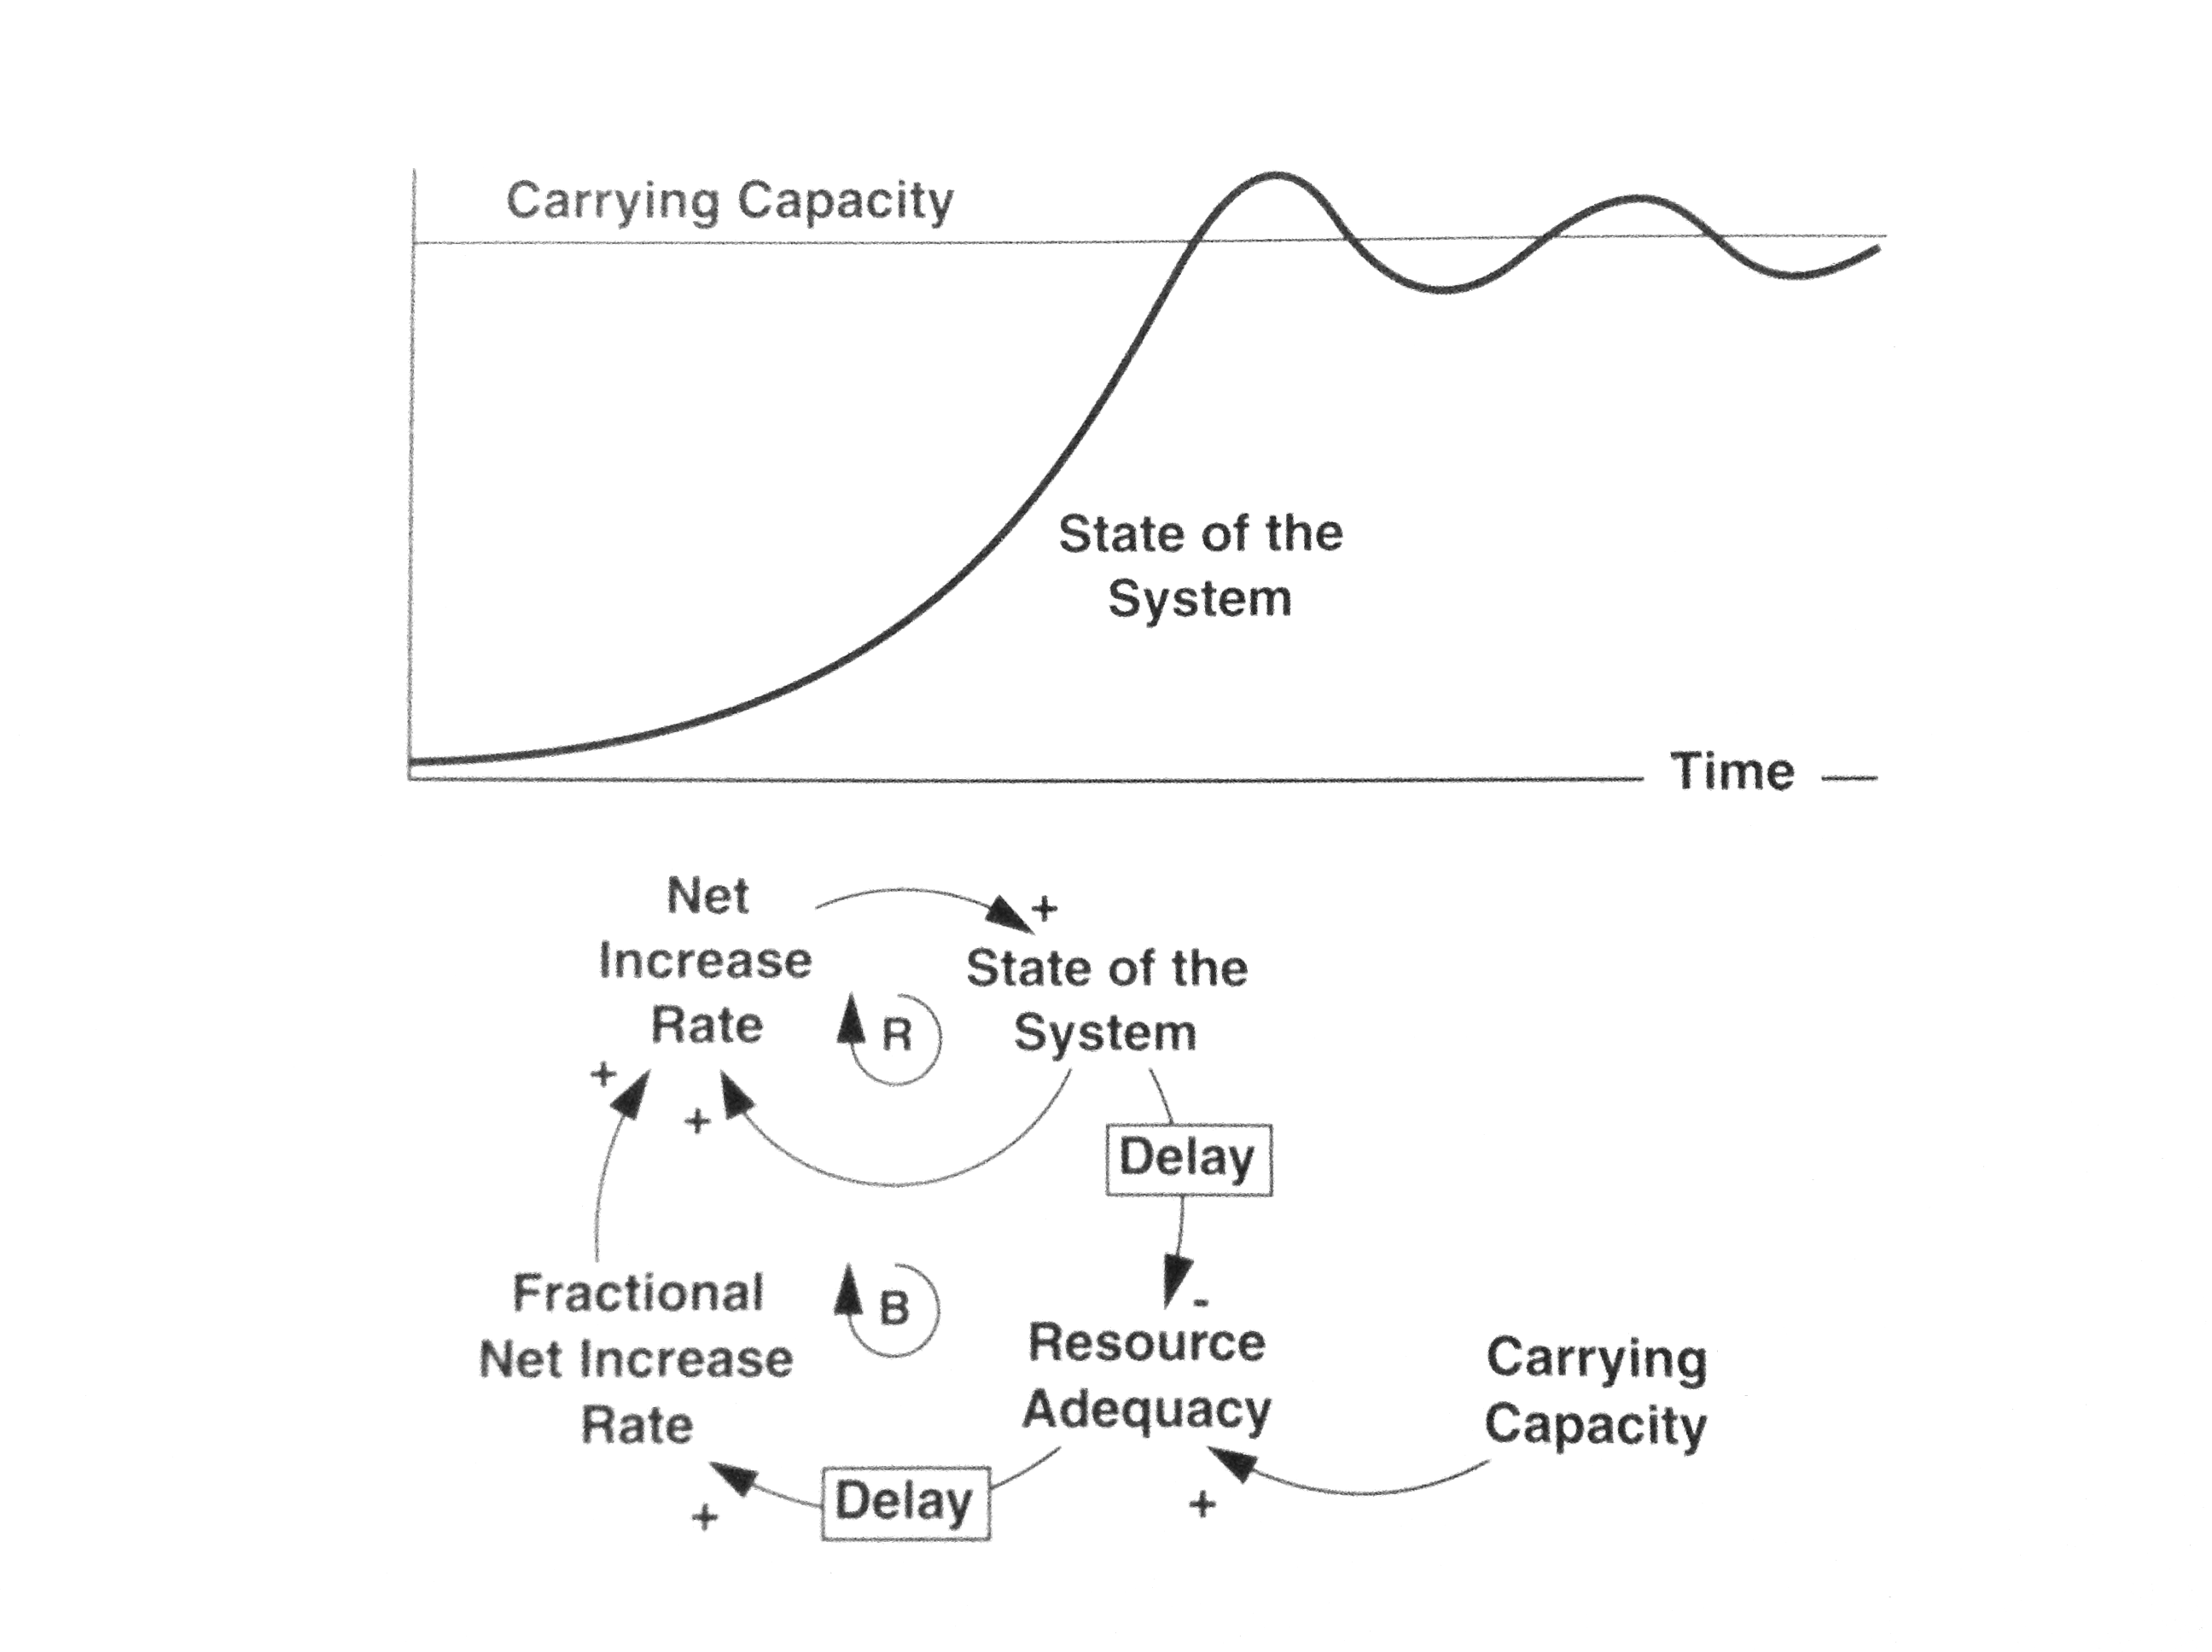
\includegraphics[width=.75\textwidth]{over.png}
	\end{center}
	\cite{sterman2000business}
\end{frame}
\note{Teised kaks stsenaariumi on S-kujuline tõus (kõige lihtsam juhtum) ning täielik kollaps}

\begin{frame}[fragile]
  \frametitle{Näide kollapsist}
	Vaatame meie süsadmini näidet. 

	\begin{enumerate}
		\item Süsadmini koormus kasvab, kuni ta teeb 80-tunniseid töönädalaid 
		\item Sellega harjutakse
		\item Admini tervis ütleb üles, ta satub haiglasse ning ei naase tööle
		\item Teil juhina on 
		\begin{itemize}
			\item Teadmuskadu admini valdusala kohta
			\note{Keegi ei dokumenteeri midagi, kui nii palju tööd teeb}
			\item Vajadus päevapealt leida \emph{kaks} uut admini
		\end{itemize}
		\item Kuni uued adminid leitakse ja käima joostakse, valitseb kaos, mis võib viia ettevõtte pankrotini
	\end{enumerate}
	Ehk, süsteemi tagasiside ei reageerinud õigeaegselt taluvuspiiri ületamisele, toimus ülereageerimine ning kas osaline või täielik kollaps. 
\end{frame}


%Arutelu koht
\begin{frame}[fragile]
  \frametitle{Arutelu koht}
		\begin{center}
			\textbf{Kuidas tuvastada jätkusuutmatust?}
		\end{center}
\end{frame}

\section{Ärimuudatused}
\begin{frame}[fragile]
  \frametitle{Ärimuudatused}
	\begin{itemize}
		\item Miks äri muutub \cite{foster2011creative} joonis ja viide. Globaliseerumise ja kommunikatsiooni vastasmõju ja efektid
		\item Mida teha muutuse korral
		\begin{itemize}
			\item Mis põhjustab ärimuutuse?
			\item Milles muutus seisneb (neid kahte tuleb omavahel valideerida kuid 100\% vastavust ära oota!)?
			\item Millistes organisatsiooni kihtides on muutus struktuurne ja millistes mitte (parameetrid või arhitektuur)? Arhitektuuri muutmine on kallis, parameetrite muutmine odav
			\item Kes kontrollib muutust?
			\item Milline on muutuste kadents?
		\end{itemize}

	\end{itemize}
\end{frame}

%Arutelu koht
\begin{frame}[fragile]
  \frametitle{Arutelu koht}
		\begin{center}
			\textbf{3. küsimus}
		\end{center}
\end{frame}

\begin{frame}[fragile]
  \frametitle{Keerukus}
	\begin{itemize}
		\item Miks on see oluline. Sest süsteemiteooriast rääkida ei jõua, räägime millestki praktilisest
		\item Keerukuse mõiste. Staatiline ja dünaamiline keerukus
		\item Arthur Ganson Machine with Concrete kui eksponendi näide
		\item Keerukuse eksponentsiaalne kasv üle võimete piiri
	\end{itemize}
\end{frame}



%Arutelu koht
\begin{frame}[fragile]
  \frametitle{Arutelu koht}
		\begin{center}
			\textbf{4. küsimus}
		\end{center}
\end{frame}

\begin{frame}[fragile]
  \frametitle{Näited}
	\begin{itemize}
		\item British Steel
		\item Pank
		\item \url{http://www.wired.com/2014/12/disappearing-business-of-design} näide ärimuutustest. Tehnilise kihi piirilt üles ja alla tagasi
	\end{itemize}
\end{frame}

\begin{frame}[fragile]
  \frametitle{British Steel}
	\begin{itemize}
		\item 1975. aastal pidi British Steel Corporation otsustama, kas ja kui mitu uudse tehnoloogiaga tehast Korfi korporatsioonilt osta 
		\item Granada Television filmis kogu protsessi
		\item Filmis jookseb korduvalt läbi fraas "kas üks või kaks tehast"
		\item Strateegiline analüüs näitas, et tehast ei pruugi üldse vaja olla
		\item Lõppotsus: osta kaks uue tehnoloogiaga tehast
		\item Neist üks pandi püsti kuid konserveeriti kohe. Teist ei pandud kunagi püsti ning müüdi alles mõned aastad tagasi
	\end{itemize}
	\begin{center}
		\textbf{Moraal:} ära kunagi eelda, et otsustusprotsess on ratsionaalne
	\end{center}
\end{frame}


%Arutelu koht
\begin{frame}[fragile]
  \frametitle{Arutelu koht}
		\begin{center}
			\textbf{5. küsimus}
		\end{center}
\end{frame}

\section{Riskijuhtimine}
%Arutelu koht
\begin{frame}[fragile]
  \frametitle{Arutelu koht}
		\begin{center}
			\textbf{6. küsimus}
		\end{center}
\end{frame}


\section{Viited}

\begin{frame}[t,allowframebreaks,]
  	\bibliographystyle{plainnat}
	\bibliography{it_strateegia} 

\end{frame}

%\plain{Küsimusi?}
\begin{frame}[plain]
	\begin{center}Küsimusi?\end{center}
\end{frame}


\end{document}